\documentclass[]{article}
\usepackage{amssymb}
\usepackage{amstext}
\usepackage{amsmath}
\usepackage{amsthm}
\usepackage{graphicx} 
\usepackage{hyperref}

\newtheorem*{theorem}{Theorem}
\newtheorem*{definition}{Definition}
\newtheorem*{claim}{Claim}

%opening
\title{Neural Networks Can Approximate Continuous Functions}
%\author{Paul Dubois}
\date{}

\begin{document}

\maketitle

\begin{abstract}
	A clean Tex version of the proof seen during the lectures that neural networks with ReLU activation can approximate continuous functions.
\end{abstract}

\section{Statement}
\begin{definition}
	$\mathcal{C}\left( \left[ a,b \right] \right)$ is the set of real continuous functions on $\left[ a,b \right]$.
\end{definition}
\begin{definition}
	$\mathcal{P}\left( n,l \right)$ is the set of rectangle 1D-1D perceptrons with $l$ hidden layers and $n$ neurons in each hidden layer.
\end{definition}

\begin{theorem}[Particular case of the universal approximation theorem\footnote{See \url{https://en.wikipedia.org/wiki/Universal_approximation_theorem} for details.}]
	$$\forall f \in \mathcal{C}(\left[ a,b \right]), \ \forall \varepsilon > 0, \ \exists N \in \mathbb{N}, \exists p \in \mathcal{P}(N,1), \|p-f\|_\infty < \varepsilon$$
	where $\|g\|_\infty$ is the infinity norm of $g$ on $\left[ a,b \right]$; i.e. $\|g\|_\infty = \max_{x \in \left[ a,b \right]}(|g(x)|)$.
\end{theorem}


\section{Idea}
The idea of the proof is to split the interval $\left[ a,b \right]$ in sub intervals such that $f$ has variation less than $\varepsilon$ in the sub-intervals.
Then, choose the weights of the neural network to interpolate linearly $f$ et the beginning and end of the sub-intervals.

A live version of this proof process is available here:
\url{https://pauldubois98.github.io/NeuralNetworkLiveProof/}.

%\newpage
%Start with a given function $f \in \left[ a,b \right]$:\newline
%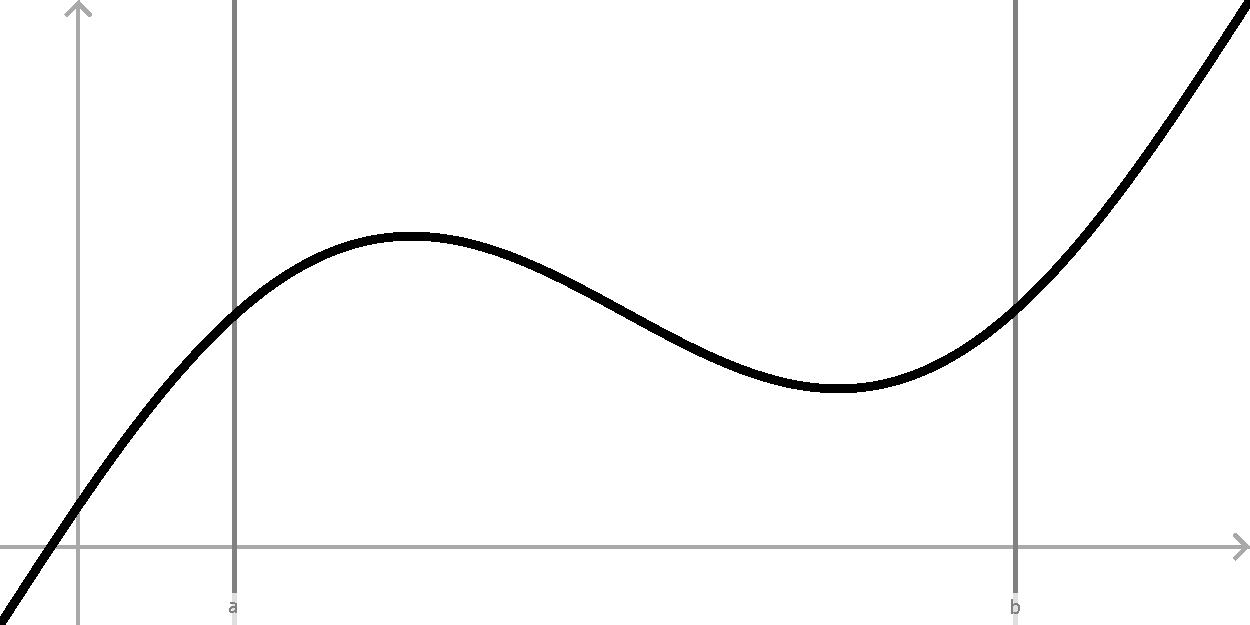
\includegraphics[width=\linewidth]{plot_1}
%\vspace{1cm}
%
%Create "boxes" of maximum height $\varepsilon$:\newline
%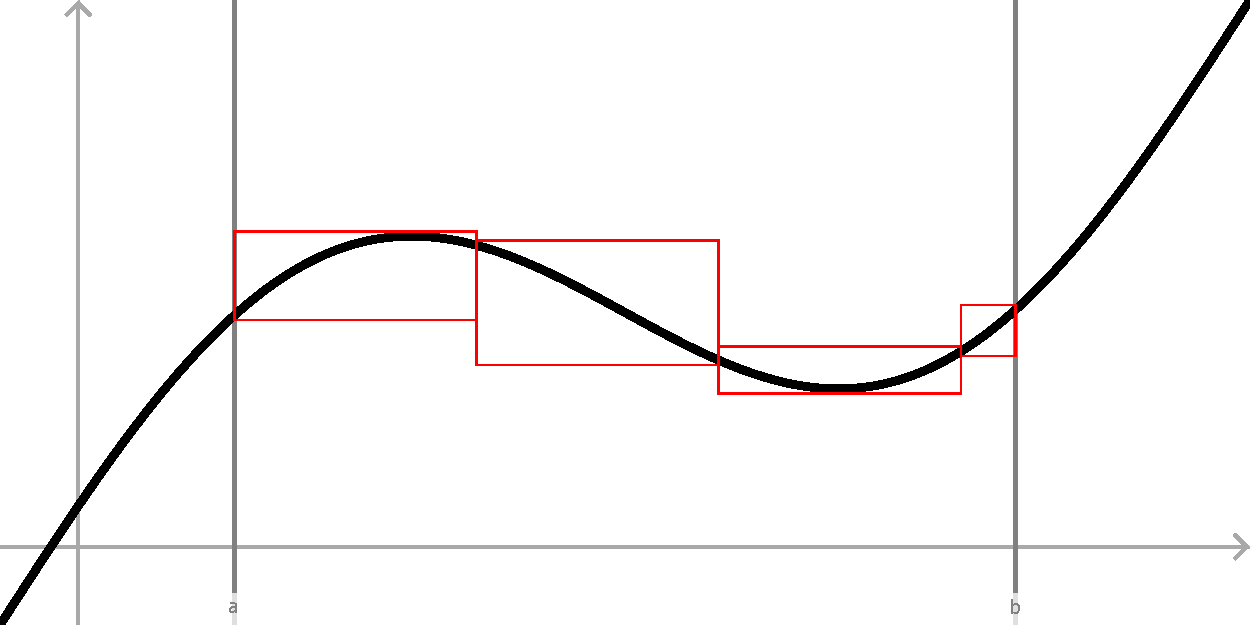
\includegraphics[width=\linewidth]{plot_2}
%\vspace{1cm}
%
%Divide the interval $\left[ a,b \right]$ in sub-intervals using the boxes:\newline
%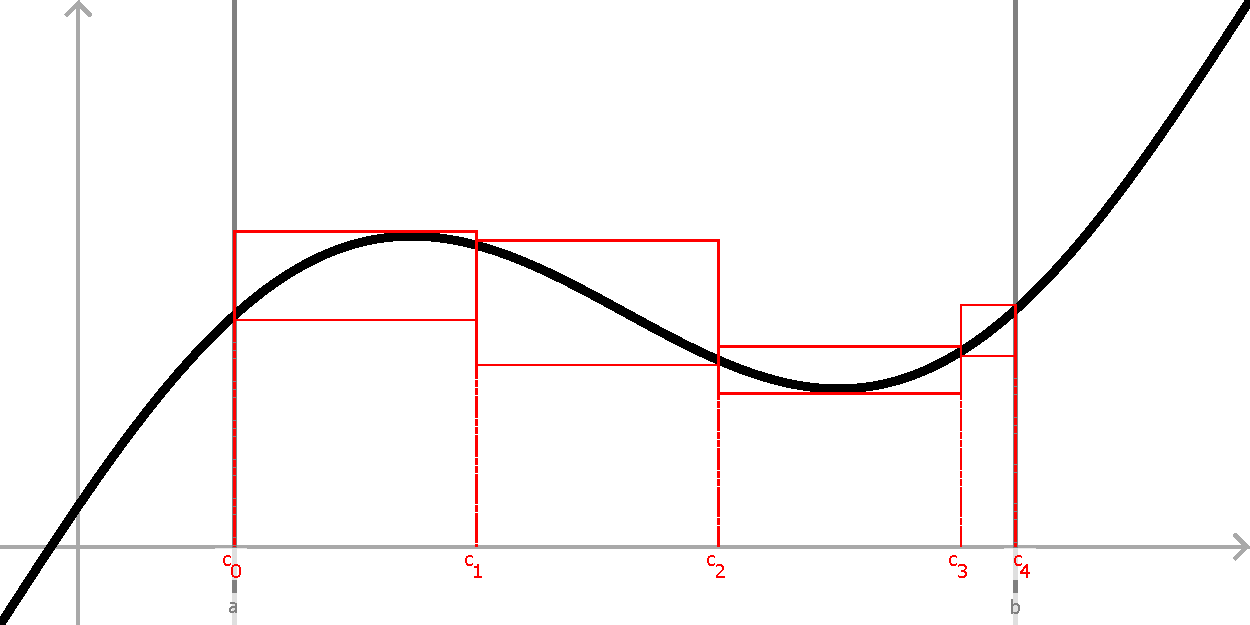
\includegraphics[width=\linewidth]{plot_3}
%\vspace{1cm}
%
%Interpolate $f$ linearly from the beginning to the end of each interval:\newline
%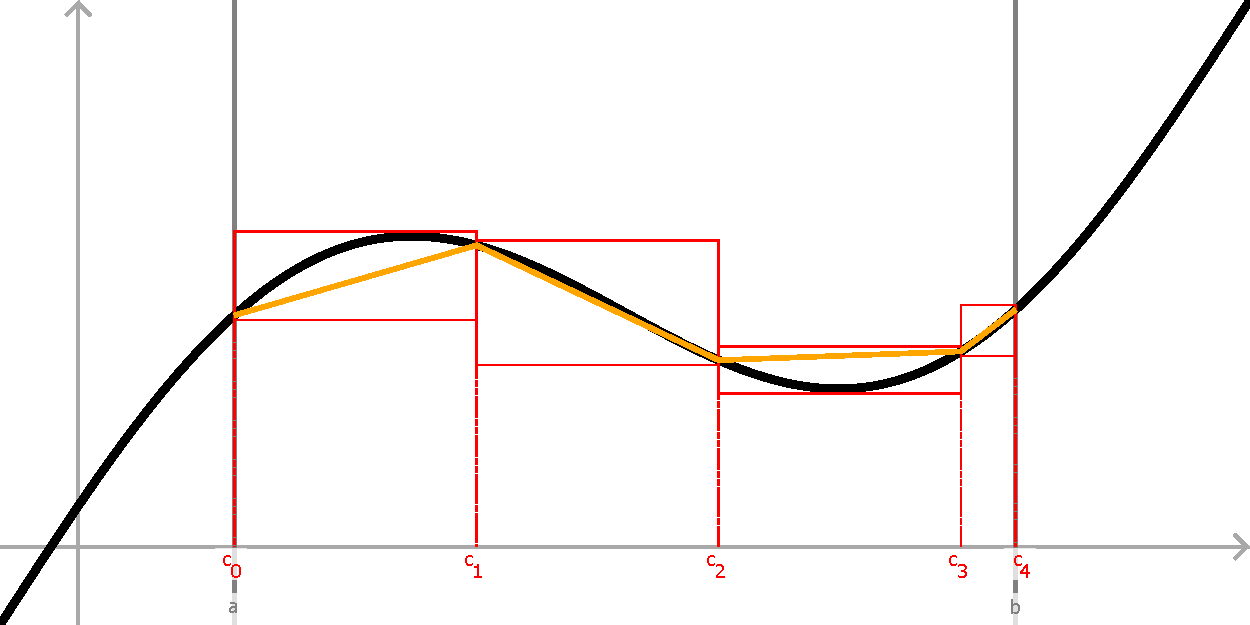
\includegraphics[width=\linewidth]{plot_4}
%\vspace{1cm}
%
%Create a network with weights that fit this interpolation:\newline
%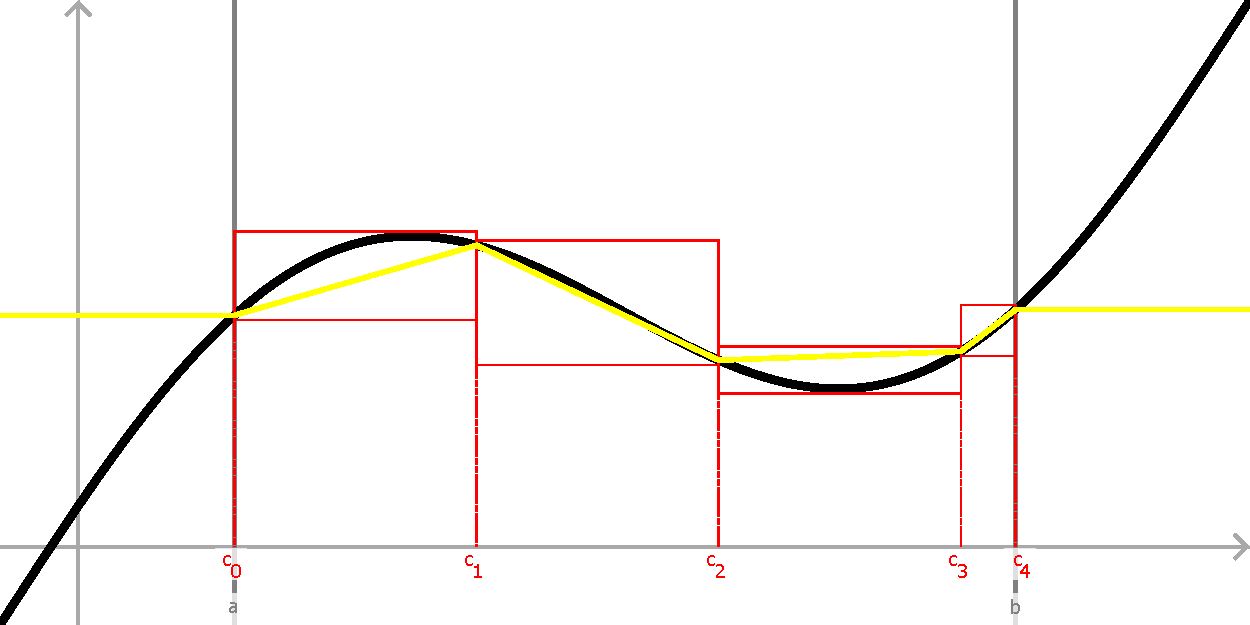
\includegraphics[width=\linewidth]{plot_5}

\section{Proof}
Let $\varepsilon >0$ and $f \in \mathcal{C}(\left[ a,b \right])$ with $a,b \in \mathbb{R}$, we want to find $N \in \mathbb{N}$ and $p \in \mathcal{P}(N,1)$ such that $\|p-f\|_\infty < \varepsilon$.

\paragraph{ReLU Network}
If $p \in \mathcal{P}(N,1)$, then 
$$p(x) = \xi + \sum_{k=0}^{N-1} \gamma_k (\alpha_k x + \beta_k)_+$$
where $(x)_+$ is $\text{ReLU}(x)$.

All we need to do is to find the right coefficients $\xi, \alpha_k, \beta_k, \gamma_k (0 \leq k < N)$ such that $\forall x \in \left[ a,b \right] |f(x)-p(x)| < \varepsilon$.

\paragraph{Uniform Continuity}
Since $f$ is continuous on a compact set, so $f$ is uniformly continuous\footnote{cf. \url{https://en.wikipedia.org/wiki/Uniform_continuity} to understand the difference between continuity and uniform continuity}.
Thus:

$$\forall x_1,x_2 \in \left[ a,b \right], \exists \delta>0,  |x_1-x_2| < \delta \implies |f(x_1) - f(x_2)| < \varepsilon.$$

\paragraph{Sub-intervals}
Let $c_0 = a$ and $c_{i+1} = c_i + \delta$. Let $N \in \mathbb{N}$ be such that $c_N \geq b$ and redefine $c_N = b$.

\paragraph{Coefficients}
Take:
\begin{itemize}
	\item $\alpha_k = 1 \quad (0 \leq k < N)$
	\item $\beta_k = -c_k \quad (0 \leq k < N)$
	\item $\tilde{\gamma_k} = \frac{f(c_{k+1})-f(c_k)}{c_{k+1}-c_k} \quad (0 \leq k < N)$
	\item $\gamma_0 = \tilde{\gamma0}$
	\item $\gamma_k = \tilde{\gamma_{k+1}} - \tilde{\gamma_k}  \quad (0 < k < N)$
	\item $\xi = f(a)$
\end{itemize}
Thus, $$p(x) = \xi + \sum_{k=0}^{N-1} \gamma_k (\alpha_k x + \beta_k)_+$$
becomes $$p(x) = f(a) + \sum_{k=0}^{N-1} \gamma_k (x - c_k)_+.$$

\paragraph{Intermediate Result}
\begin{claim}[`The network interpolates linearly from $c_n$ to $c_{n+1}$']
	If $x \in \left[ c_n, c_{n+1} \right]$, then $p(x) = f(c_n) + \tilde{\gamma_n}(x-c_n)$.
\end{claim}
\begin{proof}
	\textbf{Case $k=0$:}\newline
	Let $x \in \left[ c_0, c_1 \right]$, then:
	$$p(x) = f(a) + \sum_{k=0}^{N-1} \gamma_k (x - c_k)_+$$
	since $x \leq c_1$, $(x - c_k)_+ = 0 \quad \forall k>0$, and $(x - c_k)_+ = x - c_k$: 
	$$p(x) = f(a) + \gamma_0 (x - c_0)$$
	as $\tilde{\gamma_0} =\gamma_0$ and $a = c_0$, we finally have $p(x) = f(a) + \tilde{\gamma_0}(x - c_0)$, as expected.
	
	\textbf{Recursion:}\newline
	\begin{itemize}
		\item Suppose that if $x \in \left[ c_n, c_{n+1} \right]$, then $p(x) = f(c_n) + \tilde{\gamma_n}(x-c_n)$.
		\item We want to show that if $x \in \left[ c_{n+1}, c_{n+2} \right]$, then $p(x) = f(c_{n+1}) + \tilde{\gamma_{n+1}}(x-c_{n+1})$.
	\end{itemize}
	Let $x \in \left[ c_{n+1}, c_{n+2} \right]$, let's calculate $p(x)$:
	$$p(x) = f(a) + \sum_{k=0}^{N-1} \gamma_k (x - c_k)_+$$
	if $k > n+1$, then $c_k \geq x$, so $(x - c_k)_+ = 0$; similarly, 
	if $k \leq n+1$, then $c_k < x$, so $(x - c_k)_+ = x - c_k$ thus:
	$$p(x) = f(a) + \sum_{k=0}^{n+1} \gamma_k (x - c_k)$$
	Now, let's split $(x - c_k)$ to $(x - c_{n+1}) + (c_{n+1} - c_k)$:
	$$p(x) = f(a) + \sum_{k=0}^{n+1} \gamma_k (x - c_{n+1}) + \sum_{k=0}^{n+1} \gamma_k (c_{n+1} - c_k)$$
	We can add again $(c_{n+1} - c_k)_+$ for $n+1 < k < N$ (this is just adding zeros) to the second sum to make $p(c_{n+1})$ appear:
	$$p(x) = f(a) + \sum_{k=0}^{N-1} \gamma_k (c_{n+1} - c_k)_+ + \sum_{k=0}^{n+1} \gamma_k (x - c_{n+1})$$
	$$= f(c_{n+1}) + \sum_{k=0}^{n+1} \gamma_k (x - c_{n+1})$$
	Now, $\gamma_k = \tilde{\gamma_k} - \tilde{\gamma_{k-1}} \quad 0 < k <N$ and $\tilde{\gamma_0} = \gamma_0$, so:
	$$p(x) = f(c_{n+1}) + \gamma_0 (x - c_{n+1}) + \sum_{k=1}^{n+1} (\tilde{\gamma_k} - \tilde{\gamma_{k-1}}) (x - c_{n+1})$$
	This is a telescoping series, after simplification, we have:
	$$p(x) = f(c_{n+1}) + \tilde{\gamma_{n+1}} (x - c_{n+1})$$
	As expected.
\end{proof}
Therefore, we have that $\forall\, 0 \leq n < N$, if $x \in \left[ c_n, c_{n+1} \right]$, then $p(x) = f(c_n) + \tilde{\gamma_n}(x-c_n)$.

\paragraph{Bounds for $f$ and $p$ on $\left[ c_n, c_{n+1} \right)$}
Take $x \in \left[ c_n, c_{n+1} \right)$, then we have: $|c_n - x| < \delta$, so $|f(x) - f(c_n)| < \varepsilon$.

WLOG\footnote{Without Loss Of Generalities}, take $f(c_n) \leq f(c_{n+1})$:
- $f(c_n) \leq p(x) \leq f(c_{n+1})$ and $|f(c_{n+1}) - f(c_n)| \leq \varepsilon$ so $|p(x) - f(c_n)| \leq \varepsilon$.

\paragraph{Bound for $f - p$ on $\left[ a,b \right]$}
\begin{align*}
	\forall\, 0 \leq n < N, \ \forall\, x \in \left[ c_n, c_{n+1} \right) |f(x) - p(x)| &= |f(x) - f(c_n) + f(c_n) - p(x)| \\
	&\leq |f(x) - f(c_n)| + |p(x) - f(c_n)| \\
	&< \varepsilon + \varepsilon = 2\varepsilon
\end{align*}
Therefore it is true on $\left[ a,b \right)$.

Moreover, $p(b) = f(b)$ (from the property above), so $|f(x) - p(x)| < 2\varepsilon$ on all of $\left[ a,b \right]$.

Thus, we finally have $\|f-p\|_\infty < 2\varepsilon$.

\paragraph{Conclusion}
Now, taking $\tilde{\varepsilon} = \frac{1}{2}\varepsilon$, we get $\|f-p\|_\infty < \tilde{\varepsilon}$ with the same reasoning.

Hence, $f$ can be $\epsilon$ approximated by a single hidden layer perceptron.

\end{document}
